\documentclass[border=2pt]{standalone}
\usepackage{tikz}
\usepackage{pgfplots}
\pgfplotsset{compat=1.18}
\usepgfplotslibrary{fillbetween}

% Brand colors
\definecolor{Garnet}{rgb}{0.451, 0.0, 0.039}
\definecolor{Atlantic}{rgb}{0.275, 0.416, 0.624}
\definecolor{Horseshoe}{rgb}{0.396, 0.471, 0.043}
\definecolor{Black90}{rgb}{0.212, 0.212, 0.212}

\begin{document}
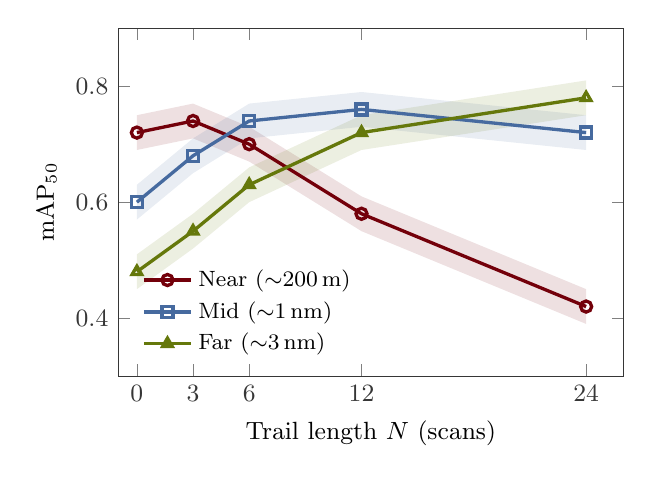
\begin{tikzpicture}
\begin{axis}[
  width=8cm,
  height=6cm,
  xmin=-1, xmax=26,
  ymin=0.3, ymax=0.9,
  xlabel={Trail length $N$ (scans)},
  ylabel={mAP$_{50}$},
  xlabel style={font=\small},
  ylabel style={font=\small},
  xtick={0,3,6,12,24},
  axis line style={Black90},
  tick label style={font=\small, color=Black90},
  legend style={
    at={(0.03,0.03)},
    anchor=south west,
    draw=none,
    fill=none,
    font=\footnotesize,
    cells={anchor=west}
  },
  rounded corners=0pt,
  every axis plot/.append style={line width=1.2pt}
]

% Near range
\addplot[color=Garnet, mark=o, mark size=2pt]
  coordinates {(0,0.72) (3,0.74) (6,0.70) (12,0.58) (24,0.42)};
\addlegendentry{Near ($\sim$200\,m)}

\addplot[name path=near_upper, draw=none, forget plot]
  coordinates {(0,0.75) (3,0.77) (6,0.73) (12,0.61) (24,0.45)};

\addplot[name path=near_lower, draw=none, forget plot]
  coordinates {(0,0.69) (3,0.71) (6,0.67) (12,0.55) (24,0.39)};

\addplot[Garnet, opacity=0.12, forget plot] fill between[of=near_upper and near_lower];

% Mid range
\addplot[color=Atlantic, mark=square, mark size=2pt]
  coordinates {(0,0.60) (3,0.68) (6,0.74) (12,0.76) (24,0.72)};
\addlegendentry{Mid ($\sim$1\,nm)}

\addplot[name path=mid_upper, draw=none, forget plot]
  coordinates {(0,0.63) (3,0.71) (6,0.77) (12,0.79) (24,0.75)};

\addplot[name path=mid_lower, draw=none, forget plot]
  coordinates {(0,0.57) (3,0.65) (6,0.71) (12,0.73) (24,0.69)};

\addplot[Atlantic, opacity=0.12, forget plot] fill between[of=mid_upper and mid_lower];

% Far range
\addplot[color=Horseshoe, mark=triangle, mark size=2pt]
  coordinates {(0,0.48) (3,0.55) (6,0.63) (12,0.72) (24,0.78)};
\addlegendentry{Far ($\sim$3\,nm)}

\addplot[name path=far_upper, draw=none, forget plot]
  coordinates {(0,0.51) (3,0.58) (6,0.66) (12,0.75) (24,0.81)};

\addplot[name path=far_lower, draw=none, forget plot]
  coordinates {(0,0.45) (3,0.52) (6,0.60) (12,0.69) (24,0.75)};

\addplot[Horseshoe, opacity=0.12, forget plot] fill between[of=far_upper and far_lower];

\end{axis}
\end{tikzpicture}
\end{document}
